Deep neural networks are often thought of as ``black boxes'' that are
easy to train but difficult to intepret. Interpreting the results
obtained using these techniques may indeed be more challenging than
getting the results themselves. This difficulty of interpretation
sometimes leads to the suspiction that the neural network learns
artifacts in the data that correlate with the target results but are
not meaningful by themselves.
%
In this section we attempt to show that our network learns relevant
description of a protein structure and does not rely on small
differences in submissions between prediction groups.
%%% GL: ``submissions between prediction groups''? I don't understand
%%% what you mean.

First, we identify the regions of a structure that are responsible for
an increase of its score (a \emph{decrease} in its quality). If the
network has learned intepretable features of the data, we expect this
analysis to show that the regions responsible for the poor quality of
a decoy structure are those in which it deviates from the native
structure.
%
We use the Grad-CAM analysis technique proposed by Selvaraju et
al.~\cite{selvaraju2016grad}. The key idea of this technique is to
propagate the gradient of the output to a certain layer of the network
and take the sum of the activations of this layer weighted by the
gradient.
%%% GL: ``Propagate'' is jargon, here. You mean you are calculating
%%% the gradient of the input w.r.t. the input to all nodes of a
%%% certain layer?
%
%%% GL: ``Activation'' is also jargon. We need to explain what it is.
%
%%% GL: Why ``activations'' plural but ``gradient'' singular?
%
%%% GL: Let me try to put that in simpler words:
This highlights all units from that layer that are both strongly
activated and highly influential on the output.
%
%%% GL: Too much jargon in the next sentence (upscaled? reception
%%% field?).
The weighted activation maps are then upscaled to the whole
reception field of the network. They indicate which parts of the
input contribute the most to the gradient of the network output.
%
In our case we choose the activations of the ReLU layer 10, for which
the activation maps are $25\times 25\times 25$.
%%% GL: This is not clear. The layer counting is not at all obvious
%%% from Figure 3 and the reader won't be able to identify which layer
%%% we're talking about.
%
%%% GL: Figure 3 needs to be more accurate. It should show all layers,
%%% as well as the size of each 3D grid. If I'm not mistaken, it goes
%%% 120x120x120, 118x118x118, 58x58x58, 56x56x56, 27x27x27, 25x25x25,
%%% 23x23x23, 11x11x11, 9x9x9, 7x7x7 (not shown!), 5x5x5, 3x3x3 (not
%%% shown!), 1x1x1.
%
We tested the method on the activation maps of neighboring layers and
layer 10 represents the best tradeoff between interpretability and
coarseness.
%%% GL: Best? Did you try other layers?
%
An example of the output is given in Fig.~\ref{Fig:GradCAMT0776}
%%% GL: Are the results for this particular target typical?
%
In line with our scoring procedure, we perform the Grad-CAM analysis
by uniformly sampling 100 rotations and translations of the decoys. We
obtain the activation maps for each of the transformations sampled and
project them onto the atoms of the
decoy. Figure~\ref{Fig:GradCAMT0776} shows two representations of such
an average activation map (for decoy Distill\_TS3 of target T0776): a
projection of the map onto the atoms of the decoy, represented as a
color-coded value on the cartoon rendering of the structure, and a
projection onto a 3D grid, represented as an isosurface. The
isosurface of Fig.~\ref{Fig:GradCAMT0776} is a hollow shell containing
most of the solvent exposed region of the decoy, which indicates that
the network enforces packing: any increase in the atomic density
around the well-packed core is penalized.
%
Strikingly, we find that the activation maps are mostly zero for
structures close to the native ones (results not shown), despite the
fact that no gradient information was included in the training
procedure. This suggests that the model has learned a score $f$ that
plays a role similar to a free energy of folding and becomes minimum
for the native structure.

Figure~\ref{Fig:GradCAMT0776_more} shows the color-coded
values of the maps for four decoys of target T0776.
%%% GL: Discussion of these results???


\begin{figure}[H]
    \centering
    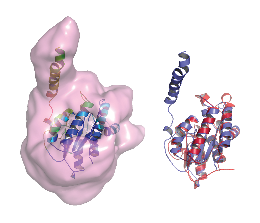
\includegraphics[width=0.5\linewidth]{Fig/FigT0776.eps}
%
    \caption{Left: Gradient-weighted activation map of the network for
    candidate structure Distill\_TS3 of target T0776. The isosurface
    shows the activation map at the two-sigma level. The intensities
    of the activation map at the positions of the protein atoms are
    color-coded on the cartoon rendering of the structure, from blue
    (low intensity) to red (high intensity). Right: Cartoon
    representation of the Distill\_TS3 decoy structure (in blue)
    aligned to the native structure (in red).}
%%% GL: Why do you say ``*scaled* gradient-weighted activation map''?
%%% The figure would look exactly the same if the maps were not
%%% scaled.
%
    \label{Fig:GradCAMT0776}
\end{figure}

\begin{figure}[H]
    \centering
    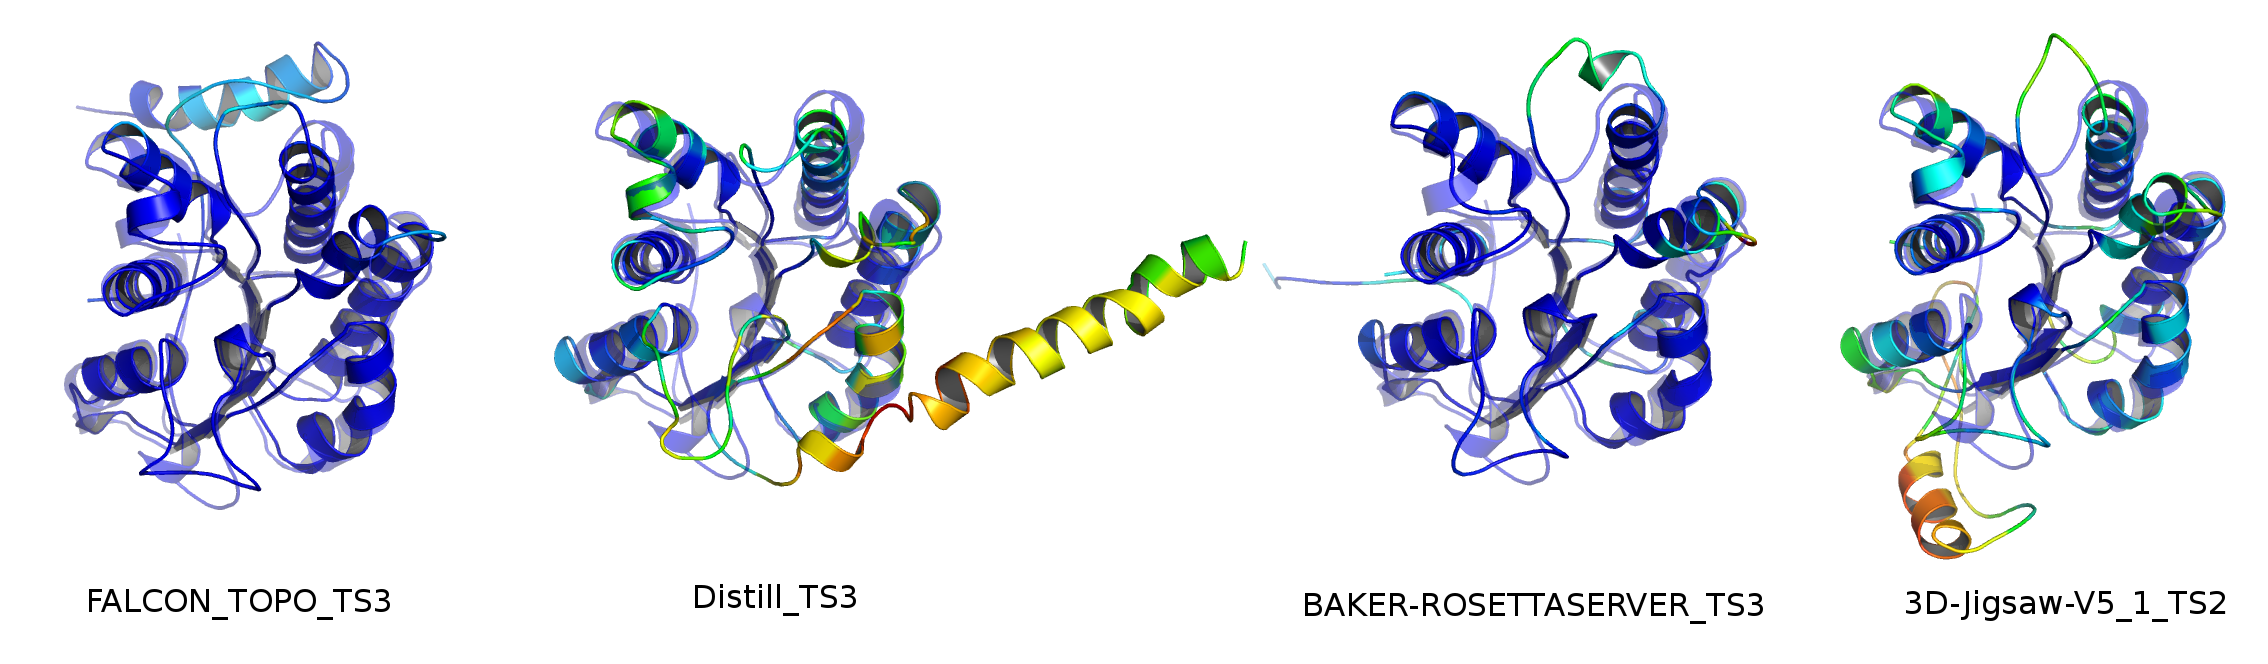
\includegraphics[width=\linewidth]{Fig/T0776.eps}
%
    \caption{Gradient-weighted activation maps of the network
    projected onto the atoms of the decoys. Each decoy is aligned to
    the native structure, shown as a transparent, blue cartoon.}
%%% GL: Why ``scaled''?
%
    \label{Fig:GradCAMT0776_more}
\end{figure}

To verify that the network we trained does not rely on artifacts in
the data to rank decoys, we have assessed its performance on a second,
independent dataset generated by the 3DRobot
algorithm \cite{deng20163drobot}. The decoys generated by this
algorithm are uniformly distributed within RMSD range of $[0; 12\AA]$
of the native structure and are optimized for the number of hydrogen
bonds and compactness.
%%% GL: What do you mean? They maximize the number of HBs and the
%%% compactness?
%
%%% GL: Why targets are you using? How many decoys per target? You
%%% need to explain better what that second dataset is.
%
The absolute \tchanged{Pearson} $R$ coefficient averaged over all the
structures in this benchmark was $0.85$. Spearman $\rho$ coefficient
and Kendall $\tau$ coefficien were $0.83$ and $0.64$, respectively.
Representative examples of scoring funnels are shown in
Fig.~\ref{Fig:3DRobotBenchmark}.  We see, that the MQA method devised
in this work successfully ranks unrelated datasets, that has the same
hyperparameters of the underlying decoys generator.
%%% GL: What do you mean? What hyperparameters? What generator?

\begin{figure}[H]
    \centering
    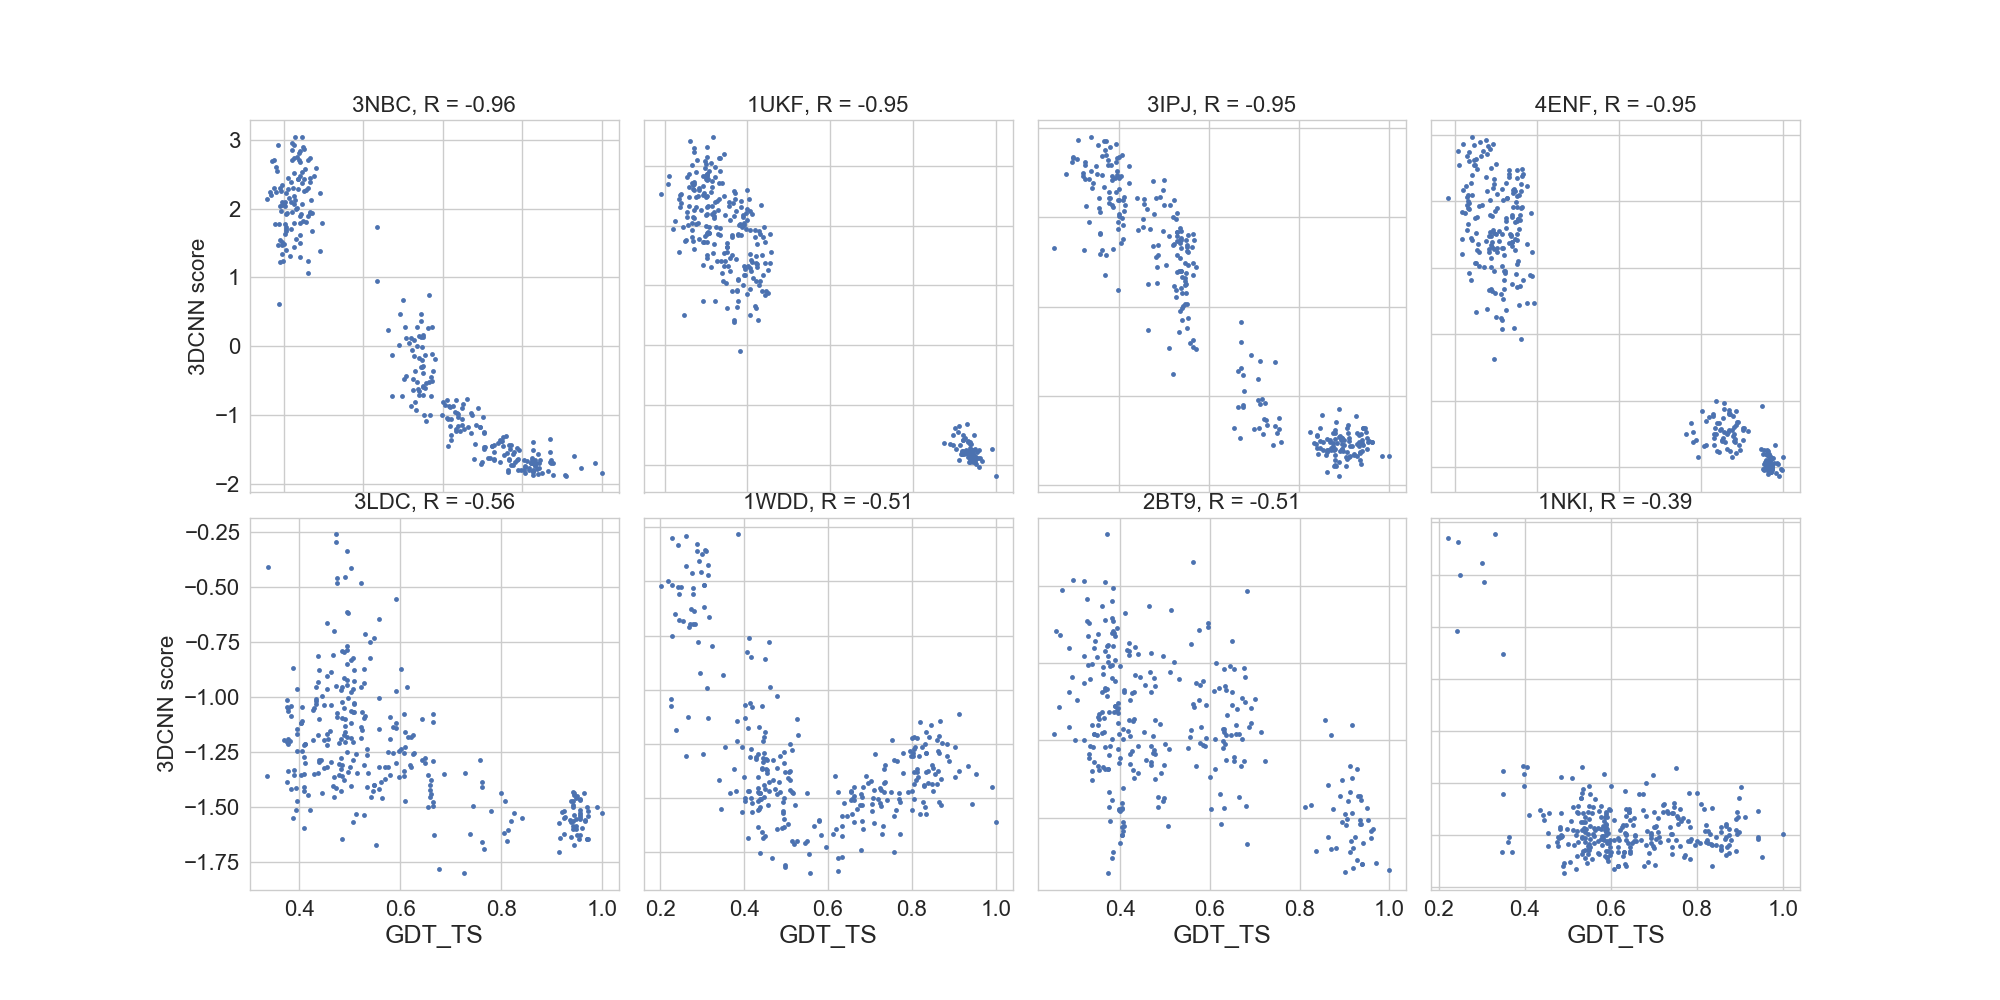
\includegraphics[width=\linewidth]{Fig/3DRobot_set_sFinal_funnels.eps}
%
    \caption{Scoring funnels of four best correlated targets and four
    least correlated targets in the 3DRobot benchmark.}
%%% GL: You don't explain what a ``scoring funnel'' is.
%
    \label{Fig:3DRobotBenchmark}
\end{figure}
